% !TeX root = ../solution.tex

\hypertarget{he22.20}{%
\chapter{[HE22.20] Coney Island Hackers}\label{he22.20}}

\begin{marginfigure}
	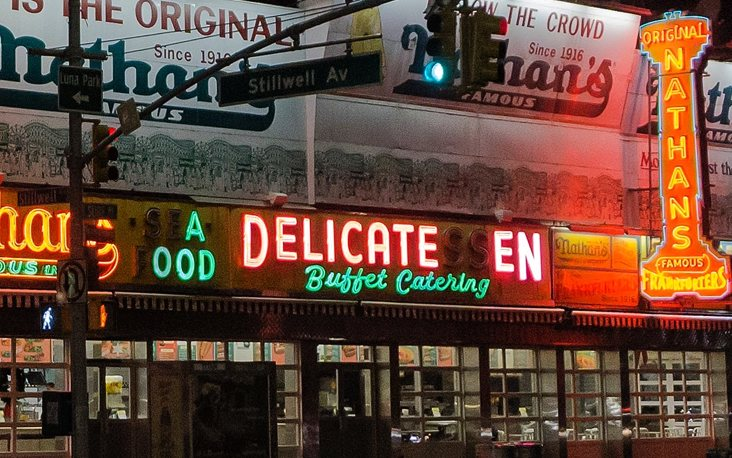
\includegraphics[width=49mm]{level5/challenge20.jpg}
\end{marginfigure}
\section{Intro}
Coney Island Hackers have a secret web portal.

Using advanced social engineering techniques, you found out their secret passphrase: \verb+eat,sleep,hack,repeat+. However, it seems to take more than just entering the passphrase as-is. Can you find out what?

\noindent \url{http://46.101.107.117:2202}

\noindent Note: The service is restarted every hour at x:00.
\subsection{Hint}

\verb+if (req.query.passphrase == 'eat,sleep,hack,repeat')+

\section{Solution}\label{hv22.20solution}

When the leaked password is entered, a message ``DANGER, commas detected' is presented.  So the task is to bypass the detection of commas in the password.  The hint given indicates that the use of the equality operator \verb+==+ is the problem here.  Reading up on the conversion rules if the two objects to be compared do not have the same type, we find that an array of strings will be converted to a comma separated string.

To create an array as part of the request, \verb+?passphrase[0]=eat&passphrase[1]=sleep,...+ can be used.  When properly HTMLized, we get the flag \verb+he2022{el_dorado_arkade}+.
	
\subsection{Notes}
\url{https://newbedev.com/passing-arrays-as-url-parameter}








